\section{Concepto de Conjunto}

El concepto de conjunto es uno de los más fundamentales y primitivos de la matemática. Intuitivamente, se entiende como una colección bien definida de objetos. Ejemplos de estos pueden ser un enjambre de abejas, los verbos, los habitantes de un barrio, entre otros.

Para formalizar este concepto y trabajar con él, primero debemos establecer ciertos elementos básicos: el contexto donde trabajamos (Universo) y las reglas para seleccionar elementos (Proposiciones).

\subsection{Fundamentos y Definiciones Básicas}

\textbf{Conjunto Universal:} \\
Cada vez que trabajemos con conjuntos, siempre estaremos referidos a un conjunto particular llamado referencial o universal, denotado usualmente como $U$. Este es el "gran conjunto" de donde se sacan los elementos. Ejemplos comunes incluyen los Naturales $\mathbb{N}$, los Enteros $\mathbb{Z}$, los Racionales $\mathbb{Q}$, los Irracionales $\mathbb{I}$ o los Reales $\mathbb{R}$.

\vspace{0.3cm}

\textbf{Funciones Proposicionales (o Predicados):} \\
Hasta ahora habíamos visto proposiciones con un valor de verdad fijo. En teoría de conjuntos, utilizamos \textit{funciones proposicionales} $p(x)$ que dependen del valor que tome la variable $x$ dentro del universo.
Por ejemplo, si tenemos la proposición ``$p(x): x \text{ es par}$'', su verdad depende de $x$:
\begin{itemize}
    \item $p(2)$ significa que $2$ es par (Verdadero).
    \item $p(1)$ significa que $1$ es par (Falso).
\end{itemize}

\subsection{Determinación de Conjuntos}

Los conjuntos los podemos presentar o determinar de dos formas principales:

\begin{enumerate}
    \item \textbf{Por Extensión:} Se hace una lista explícita de todos sus elementos.
    \item \textbf{Por Comprensión:} Se entiende el conjunto como una reunión de elementos que comparten una característica común. 
\end{enumerate}

Para definir un conjunto por comprensión de manera formal, precisamos del conjunto referencial $U$ y de una función proposicional $p(x)$. Así, diremos que $A$ es el conjunto de todos los $x$ que están en el universal $U$ que hacen verdadera a la proposición $p(x)$. Esto se escribe como:
\[ A =\{x\in U \mid p(x)\} \]

\footnotesize
\noindent \textit{Nota:} El uso estricto de un conjunto universal es vital para evitar contradicciones lógicas famosas, como la \textbf{Paradoja de Russell}. Si definiéramos conjuntos libremente sin restringirnos a un universo $U$ (por ejemplo, intentando crear ``el conjunto de todos los conjuntos que no se pertenecen a sí mismos''), llegaríamos a una contradicción irresoluble.
\normalsize

\subsection{Relación de Pertenencia}

Dado un conjunto $A = \{x\in U \mid p(x)\}$, la relación de pertenencia se define lógicamente así:

\begin{itemize}
    \item Diremos que un elemento $x$ \textbf{pertenece} al conjunto $A$, escrito como \fbox{$x\in A$}, si la proposición $p(x)$ es verdadera.
    \item Cuando la proposición $p(x)$ es falsa (o $x$ no está en $U$), diremos que $x$ \textbf{no es un elemento} de $A$ y se escribe como \fbox{$x\notin A$}.
\end{itemize}

\subsection{Ejemplos Ilustrativos y Representación}

\noindent \textbf{Ejemplo 1: Números Naturales} \\
Consideremos el conjunto de los números naturales del uno al diez.
\begin{itemize}
    \item Por extensión: $A=\{1,2,3,4,5,6,7,8,9,10\}$
    \item Por comprensión: $A = \{ x \in \mathbb{N} \mid 1 \le x \le 10 \}$
\end{itemize}
En este caso, $2 \in A$ (verdadero), mientras que $11 \notin A$ (falso).

\vspace{0.3cm}

\noindent \textbf{Ejemplo 2: Desigualdades (Intervalos)} \\
\[ B = \{x \in \mathbb{R} \mid 0\leq x \leq 2 \} \]
Se lee como: el conjunto de los números reales $x$ tales que $x$ es mayor o igual a cero y menor o igual a 2.

\vspace{0.3cm}

\noindent \textbf{Ejemplo 3: Propiedades cualitativas} \\
\[ C= \{x \mid \text{x es capital de un país suramericano} \} \]
Se lee como: los $x$ tales que $x$ es capital de un país suramericano.

\vspace{0.5cm}

\textbf{Diagramas de Venn:} \\
La representación simbólica gráfica de un conjunto se denomina Diagrama de Venn (Ver Figura \ref{fig:Venn}).

\begin{figure}[ht]
\centering
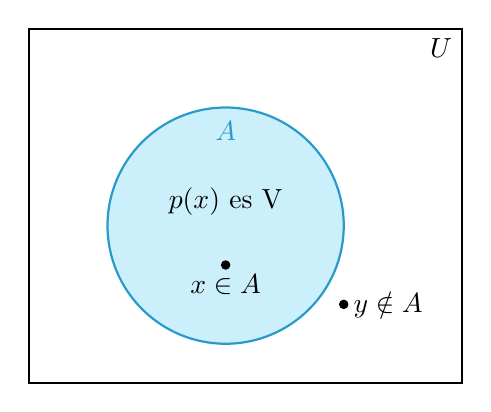
\begin{tikzpicture}
% Universal
\draw [thick] (-2.5,-2) rectangle (3,2.5);
\node [text=black, below left] at (3,2.5) {$U$};

% Conjunto A
\filldraw[cyan!20, draw=cyan!80!black, thick] (0,0) circle (1.5cm);
\node [text=cyan!80!black, font=\bfseries] at (0, 1.2) {$A$};

% Elemento x dentro de A (cumple p(x))
\node [text=black] at (0,0.3) {$p(x)$ es V};
\filldraw [black] (0,-0.5) circle (1.5pt) node[below] {$x \in A$};

% Elemento y fuera de A
\filldraw [black] (1.5,-1.0) circle (1.5pt) node[right] {$y \notin A$};
\end{tikzpicture}
\caption{Diagrama de Venn representando un conjunto $A$ dentro de un universo $U$.}\label{fig:Venn}
\end{figure}

A continuación presentamos las operaciones entre conjuntos como la unión, la intersección, el complemento y la diferencia simétrica.

\subsection{Operaciones con Conjuntos}

\subsubsection{Complemento}

Dada una función proposicional $p(x)$ y un conjunto universal $U$, sabemos que la proposición selecciona elementos para formar un conjunto $A = \{x \in U \mid p(x)\}$.

El \textbf{complemento} de $A$ es el conjunto formado por todos los elementos del referencial $U$ que \textbf{no} satisfacen la proposición $p(x)$. En términos lógicos, corresponde a la negación de la proposición original ($\neg p(x)$).

Se denota usualmente como $\bar{A}$, $A^c$ o $A'$. Formalmente:
\[ A' = \{ x\in U \mid \neg p(x) \} \]
O equivalentemente:
\[ A' = \{ x \in U \mid x \notin A \} \]

En la Figura \ref{figura:complemento}, el área sombreada representa a $A'$, es decir, todo lo que está fuera de $A$ pero dentro del universo.

\begin{figure}[ht]
\centering
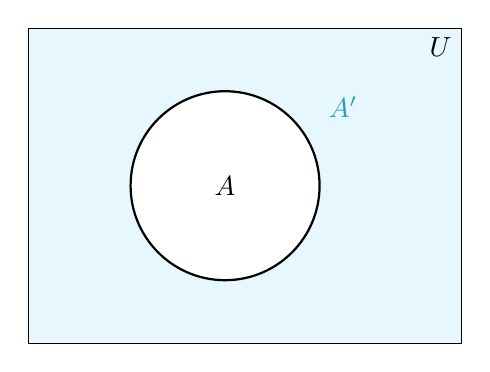
\begin{tikzpicture}
% Universal relleno (representando el complemento)
\filldraw[fill=cyan!10] (-2.5,-2) rectangle (3,2);
\node [text=black, below left] at (3,2) {$U$};

% Conjunto A (blanco para resaltar que no es parte del complemento)
\filldraw[fill=white, draw=black, thick] (0,0) circle (1.2cm);
\node [text=black, font=\bfseries] at (0,0) {$A$};

% Etiqueta del complemento
\node [text=cyan!80!black] at (1.5,1) {$A'$};
\end{tikzpicture}
\caption{Representación del Complemento ($A'$): la región sombreada.}\label{figura:complemento}
\end{figure}

\noindent \textbf{Ejemplo:}
Sea el conjunto universal $U$ definido sobre los naturales:
\[ U=\{x \in \mathbb{N} \mid 0\leq x \leq 20 \} \]
Y sea el conjunto $A$ definido como:
\[ A=\{x\in U \mid x \text{ es un número par}\} \]
Entonces, el complemento de $A$ está formado por los elementos de $U$ que hacen falsa la proposición ``es par''. Es decir:
\[ A'= \{x\in U \mid x \text{ es un número impar}\} \]
Es importante notar una propiedad fundamental: la unión de un conjunto con su complemento reconstituye el universo ($A \cup A' = U$).

\subsubsection*{Nota sobre el Conjunto Vacío}

Existe un caso especial: ¿qué pasa si la proposición $p(x)$ es siempre falsa para todos los elementos del Universo? (Por ejemplo: $x \in \mathbb{N}$ tal que $x < 0$).

En este caso, el conjunto resultante no tiene elementos. Se denomina \textbf{conjunto vacío} y se denota por el símbolo $\emptyset$ o por llaves vacías $\{ \}$.
\[ \emptyset = \{ x \in U \mid x \neq x \} \]

\noindent \textbf{Advertencias importantes:}
\begin{itemize}
    \item La proposición $x \in \emptyset$ siempre es \textbf{falsa}.
    \item El conjunto $A=\{\emptyset\}$ \textbf{no es vacío}; es un conjunto que contiene un elemento (ese elemento es el conjunto vacío).
    \item Relación con el complemento: El complemento del conjunto Universal es el conjunto vacío ($U' = \emptyset$) y viceversa ($\emptyset' = U$).
\end{itemize}

\subsubsection{Cuantificadores Lógicos}

En la definición de conjuntos y proposiciones, frecuentemente necesitamos especificar si una propiedad se cumple para \textit{todos} los elementos o si solo \textit{algunos} (o al menos uno) la cumplen. Para esto utilizamos los cuantificadores.

\paragraph{1. Cuantificador Universal ($\forall$)}
Se utiliza cuando deseamos afirmar que una proposición es verdadera para \textbf{todos} los elementos de un conjunto. El símbolo $\forall$ se lee como ``para todo'' o ``para cada''.

\noindent \textbf{Ejemplo:}
Sea el conjunto $A=\{ 2,4,6,8\}$. Podemos afirmar:
\[ \forall x \in A, \quad x \text{ es par} \]
Esto se lee: ``Para todo elemento $x$ que pertenece a $A$, $x$ es par''. Si existiera al menos un elemento en $A$ que no fuera par, esta afirmación sería falsa.

\paragraph{2. Cuantificador Existencial ($\exists$)}
Se utiliza cuando queremos indicar que \textbf{existe al menos un} elemento en el conjunto que cumple con la propiedad dada. El símbolo $\exists$ se lee como ``existe'' o ``hay al menos un''.

\noindent \textbf{Ejemplo:}
Sea el conjunto $B=\{ 1,2,4,6,8\}$. Podemos afirmar:
\[ \exists x \in B \mid x \text{ es impar} \]
Esto se lee: ``Existe un elemento $x$ en $B$ tal que $x$ es impar''. Esta proposición es verdadera porque el número $1$ pertenece a $B$ y es impar.

\vspace{0.3cm}

\noindent \textbf{Negación de Cuantificadores (Leyes de De Morgan para cuantificadores):}
Es crucial entender la relación entre ambos:
\begin{itemize}
    \item Negar que ``todos cumplen'' equivale a decir que ``existe al menos uno que no cumple''.
    \[ \neg (\forall x \in A, p(x)) \iff \exists x \in A \mid \neg p(x) \]
    \item Negar que ``existe alguno'' equivale a decir que ``ninguno cumple'' (o todos no cumplen).
    \[ \neg (\exists x \in A \mid p(x)) \iff \forall x \in A, \neg p(x) \]
\end{itemize}

\subsubsection{Inclusión y Subconjuntos}

Diremos que un conjunto $A$ está incluido en un conjunto $B$ (o que $A$ es subconjunto de $B$), si todos los elementos de $A$ pertenecen también a $B$. Se denota como \fbox{$A \subseteq B$}.

En términos de cuantificadores y lógica, la definición formal es:
\[ A \subseteq B \iff \forall x (x \in A \implies x \in B) \]
Esto se lee: ``$A$ es subconjunto de $B$ si y solo si para todo $x$, si $x$ pertenece a $A$, entonces $x$ necesariamente pertenece a $B$''.

\vspace{0.2cm}
\noindent \textbf{Propiedades Importantes:}
\begin{itemize}
    \item Todo conjunto es subconjunto de sí mismo: $A \subseteq A$.
    \item El conjunto vacío es subconjunto de cualquier conjunto: $\emptyset \subseteq A$.
\end{itemize}
\noindent \textbf{Demostración de que $\emptyset \subseteq A$ para cualquier conjunto $A$:}

\begin{proof}
Debemos probar que $\forall x (x \in \emptyset \implies x \in A)$ es verdadera.

Recordemos que la implicación lógica $P \implies Q$ es \textit{falsa} únicamente cuando $P$ es verdadero y $Q$ es falso. En todos los demás casos, la implicación es verdadera.

Ahora bien, por la definición del conjunto vacío, sabemos que la proposición ``$x \in \emptyset$'' es siempre \textbf{falsa}, sin importar qué elemento $x$ consideremos.

Por lo tanto, en la implicación $x \in \emptyset \implies x \in A$:
\begin{itemize}
    \item La hipótesis ($x \in \emptyset$) es falsa.
    \item Cuando la hipótesis de una implicación es falsa, la implicación completa es \textbf{verdadera}, independientemente del valor de verdad de la conclusión.
\end{itemize}

Este tipo de verdad se denomina \textbf{verdad vacua} (o verdad por vacuidad): una implicación cuya hipótesis nunca se satisface es automáticamente verdadera.

Como la proposición $x \in \emptyset \implies x \in A$ es verdadera para todo $x$, concluimos que $\emptyset \subseteq A$.
\end{proof}

En la Figura \ref{fig:subconjunto} se ilustra visualmente la relación de inclusión. Si existiera al menos un elemento en $A$ que no estuviera en $B$, entonces $A$ no sería subconjunto de $B$ ($A \not\subseteq B$).

\begin{figure}[ht]
\centering
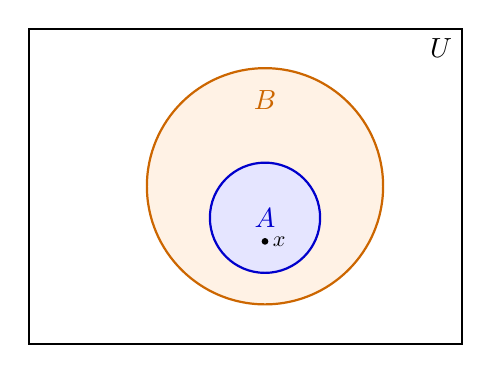
\begin{tikzpicture}
% Universal
\draw [thick] (-2.5,-2) rectangle (3,2);
\node [text=black, below left] at (3,2) {$U$};

% Conjunto B (Grande)
\filldraw[fill=orange!10, draw=orange!80!black, thick] (0.5,0) circle (1.5cm);
\node [text=orange!80!black, font=\bfseries] at (0.5,1.1) {$B$};

% Conjunto A (Pequeño, dentro de B)
\filldraw[fill=blue!10, draw=blue!80!black, thick] (0.5,-0.4) circle (0.7cm);
\node [text=blue!80!black, font=\bfseries] at (0.5,-0.4) {$A$};

% Elemento x visual
\filldraw [black] (0.5,-0.7) circle (1pt) node[right, scale=0.8] {$x$};
\end{tikzpicture}
\caption{Representación gráfica de la inclusión $A \subseteq B$.}\label{fig:subconjunto}
\end{figure}

\noindent \textbf{Ejemplo de inclusión:}
Definamos el conjunto $B$ sobre los naturales:
\[ B=\{x \in \mathbb{N} \mid 0 < x < 100 \} \]
Y el conjunto $A$ de números primos pequeños:
\[ A=\{x \in \mathbb{N} \mid x \text{ es primo } \land x \le 20 \} \]
Claramente $A \subseteq B$, ya que todos los números primos menores a 20 ($2, 3, 5, \dots, 19$) son también números naturales menores a 100.

\vspace{0.5cm}

\subsubsection{Cardinalidad y Conjunto de Partes}

\textbf{Cardinalidad:} \\
El cardinal de un conjunto es el número de elementos que contiene. Se denota usualmente con el símbolo $\#$ o con barras de valor absoluto. Por ejemplo, si $A=\{a, e, i, o, u\}$, su cardinal es $\#A=5$.

\textbf{Conjunto de Partes (Conjunto Potencia):} \\
Dado un conjunto $A$, el conjunto de partes de $A$, denotado como $\mathcal{P}(A)$, es el conjunto formado por \textbf{todos los subconjuntos posibles} de $A$ (incluyendo al conjunto vacío y al propio $A$).

\noindent \textbf{Ejemplo:}
Sea $A=\{a,b,c\}$. Su conjunto de partes es:
\[ \mathcal{P}(A) = \{ \emptyset, \{a\}, \{b\}, \{c\}, \{a,b\}, \{a,c\}, \{b,c\}, \{a,b,c\} \} \]

\noindent \textbf{Relación entre Cardinal y Potencia:} \\
Si un conjunto $A$ tiene $n$ elementos ($\#A=n$), entonces su conjunto de partes tendrá $2^n$ elementos.
\[ \#\mathcal{P}(A) = 2^{\#A} \]
En el ejemplo anterior, como $\#A=3$, verificamos que el conjunto de partes tiene $2^3=8$ elementos.

\subsubsection{Unión de Conjuntos}

Dados dos conjuntos $A$ y $B$, la unión es el conjunto formado por todos los elementos que pertenecen a $A$, a $B$, o a ambos.

Si definimos los conjuntos mediante proposiciones como $A=\{ x\in U \mid p(x)\}$ y $B=\{ x\in U \mid q(x)\}$, la unión corresponde lógicamente a la disyunción ($\lor$). Es decir, $x \in A \cup B$ si la proposición compuesta $p(x) \lor q(x)$ es verdadera.

Formalmente:
\[ A \cup B = \{ x \in U \mid x \in A \lor x \in B \} \]

En la Figura \ref{fig:union}, el área sombreada representa la unión completa de ambos conjuntos.

\begin{figure}[ht]
\centering
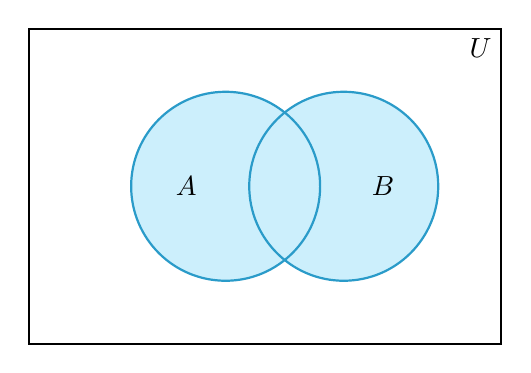
\begin{tikzpicture}
% Universal
\draw [thick] (-2.5,-2) rectangle (3.5,2);
\node [text=black, below left] at (3.5,2) {$U$};

% Conjunto A y B unidos (relleno total)
\fill[cyan!20] (0,0) circle (1.2cm);
\fill[cyan!20] (1.5,0) circle (1.2cm);

% Contornos
\draw [thick, cyan!80!black] (0,0) circle (1.2cm);
\draw [thick, cyan!80!black] (1.5,0) circle (1.2cm);

% Etiquetas
\node [text=black] at (-0.5,0) {$A$};
\node [text=black] at (2,0) {$B$};
\end{tikzpicture}
\caption{Representación gráfica de la Unión $A \cup B$.}\label{fig:union}
\end{figure}

\noindent \textbf{Ejemplo:}
Sean los conjuntos $A=\{1,2,3,4,5,6\}$ y $B=\{3,5,7,8,9,10,2\}$.
La unión entre $A$ y $B$ agrupa todos los elementos sin repetir:
\[ A\cup B=\{1,2,3,4,5,6,7,8,9,10\} \]

\vspace{0.5cm}

\subsubsection{Intersección de Conjuntos}

La intersección de dos conjuntos $A$ y $B$ es el conjunto formado únicamente por los elementos que pertenecen \textbf{simultáneamente} a ambos conjuntos.

Lógicamente, corresponde a la conjunción ($\land$). Un elemento $x \in A \cap B$ si hace que la proposición compuesta $p(x) \land q(x)$ sea verdadera.

Formalmente:
\[ A \cap B = \{ x \in U \mid x \in A \land x \in B \} \]

\begin{figure}[ht]
\centering
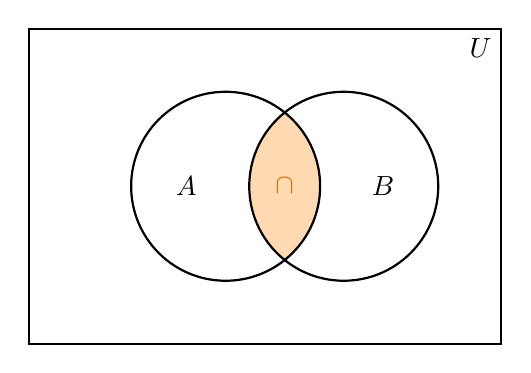
\begin{tikzpicture}
% Universal
\draw [thick] (-2.5,-2) rectangle (3.5,2);
\node [text=black, below left] at (3.5,2) {$U$};

% Relleno solo en la intersección (clip)
\begin{scope}
    \clip (0,0) circle (1.2cm);
    \fill[orange!30] (1.5,0) circle (1.2cm);
\end{scope}

% Contornos
\draw [thick, black] (0,0) circle (1.2cm);
\draw [thick, black] (1.5,0) circle (1.2cm);

% Etiquetas
\node [text=black] at (-0.5,0) {$A$};
\node [text=black] at (2,0) {$B$};
\node [text=orange!80!black] at (0.75,0) {$\cap$};
\end{tikzpicture}
\caption{Representación gráfica de la Intersección $A \cap B$.}\label{fig:interseccion}
\end{figure}

\noindent \textbf{Ejemplo:}
Sean $A=\{3,4,5,10\}$ y $B=\{1,2,3,5,8\}$.
La intersección está formada por los elementos comunes:
\[ A\cap B=\{3,5\} \]

\vspace{0.3cm}

\noindent \textbf{Conjuntos Disjuntos:}
Cuando dos conjuntos no tienen ningún elemento en común, se dice que son \textit{disjuntos} o mutuamente excluyentes. En este caso, su intersección es el conjunto vacío:
\[ A \cap B = \emptyset \]

\begin{figure}[ht]
\centering
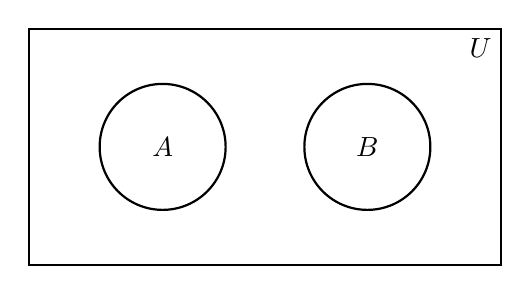
\begin{tikzpicture}
% Universal
\draw [thick] (-2.5,-1.5) rectangle (3.5,1.5);
\node [text=black, below left] at (3.5,1.5) {$U$};

% Círculos separados
\filldraw[fill=white, draw=black, thick] (-0.8,0) circle (0.8cm) node {$A$};
\filldraw[fill=white, draw=black, thick] (1.8,0) circle (0.8cm) node {$B$};
\end{tikzpicture}
\caption{Conjuntos Disjuntos ($A \cap B = \emptyset$).}\label{fig:disjuntos}
\end{figure}

\noindent \textbf{Ejemplo de disjuntos:}
Sea $A=\{3,5,7,9\}$ (impares) y $B=\{2,4,6,8\}$ (pares).
Como no comparten elementos:
\[ A\cap B=\emptyset \]
\footnotesize
\textit{Nota importante:} Matemáticamente es incorrecto escribir $\{\emptyset\}$ como resultado, pues eso sería un conjunto que contiene un elemento (el vacío), mientras que el resultado correcto es la ausencia total de elementos.
\normalsize

\subsubsection{Diferencia de Conjuntos}

La diferencia entre dos conjuntos $A$ y $B$, denotada como $A - B$ (o a veces $A \setminus B$), es el conjunto formado por todos los elementos que pertenecen a $A$ pero que \textbf{no} pertenecen a $B$.

Formalmente se define como:
\[ A - B = \{ x \in U \mid x \in A \land x \notin B \} \]

En la Figura \ref{fig:diferencia}, el área sombreada representa $A - B$ (lo que es ``exclusivo'' de A).

\begin{figure}[ht]
\centering
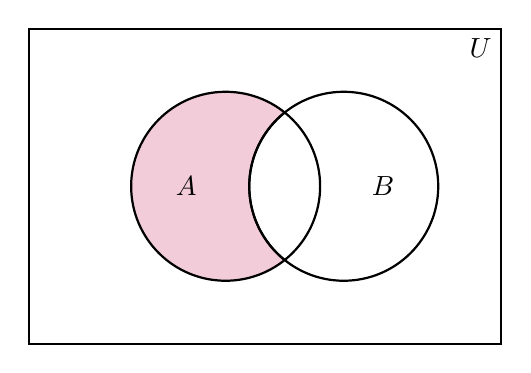
\begin{tikzpicture}
% Universal
\draw [thick] (-2.5,-2) rectangle (3.5,2);
\node [text=black, below left] at (3.5,2) {$U$};

% Diferencia A - B
\begin{scope}
    \clip (0,0) circle (1.2cm);      % Recortamos dentro de A
    \fill[purple!20] (0,0) circle (1.2cm); % Rellenamos A
    \fill[white] (1.5,0) circle (1.2cm);   % Borramos la parte de B
    \draw [thick, black] (1.5,0) circle (1.2cm); % Redibujamos contorno B
\end{scope}

% Contornos completos para asegurar visualización
\draw [thick, black] (0,0) circle (1.2cm);
\draw [thick, black] (1.5,0) circle (1.2cm);

% Etiquetas
\node [text=black] at (-0.5,0) {$A$};
\node [text=black] at (2,0) {$B$};
\end{tikzpicture}
\caption{Representación de la Diferencia $A - B$ (Elementos exclusivos de A).}\label{fig:diferencia}
\end{figure}

\noindent \textbf{Ejemplo:}
Consideremos los conjuntos:
\[ A=\{1,3,5,7,9\} \]
\[ B=\{1,2,3,4,5,6,7,8\} \]

\begin{itemize}
    \item Si calculamos $B - A$ (elementos que están en $B$ y no en $A$):
    \[ B - A = \{2, 4, 6, 8\} \]
    \item Si calculamos $A - B$ (elementos que están en $A$ y no en $B$):
    \[ A - B = \{9\} \]
\end{itemize}
Esto demuestra que la diferencia \textbf{no es conmutativa} ($A - B \neq B - A$).

\vspace{0.5cm}

\subsubsection{Diferencia Simétrica}

La diferencia simétrica entre dos conjuntos $A$ y $B$, denotada por $A \Delta B$, es el conjunto de elementos que pertenecen a $A$ o a $B$, pero \textbf{no a ambos simultáneamente}.

Se puede definir de dos formas equivalentes:
\begin{enumerate}
\item Como la unión de las diferencias: $(A - B) \cup (B - A)$
\item  Como la unión menos la intersección: $(A \cup B) - (A \cap B)$
\end{enumerate}
Formalmente:
\[ A \Delta B = \{ x \in U \mid (x \in A \land x \notin B) \lor (x \in B \land x \notin A) \} \]

\begin{figure}[ht]
\centering
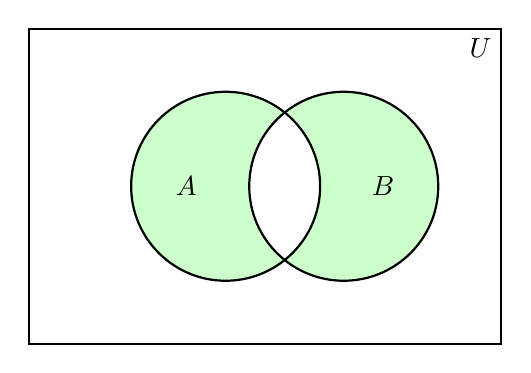
\begin{tikzpicture}
% Universal
\draw [thick] (-2.5,-2) rectangle (3.5,2);
\node [text=black, below left] at (3.5,2) {$U$};

% Diferencia Simétrica (Rellenamos todo y borramos intersección)
\fill[green!20] (0,0) circle (1.2cm);
\fill[green!20] (1.5,0) circle (1.2cm);

% Borrar intersección
\begin{scope}
    \clip (0,0) circle (1.2cm);
    \fill[white] (1.5,0) circle (1.2cm);
\end{scope}

% Contornos
\draw [thick, black] (0,0) circle (1.2cm);
\draw [thick, black] (1.5,0) circle (1.2cm);

% Etiquetas
\node [text=black] at (-0.5,0) {$A$};
\node [text=black] at (2,0) {$B$};
\end{tikzpicture}
\caption{Representación de la Diferencia Simétrica $A \Delta B$.}\label{fig:simetrica}
\end{figure}

\noindent \textbf{Ejemplo:}
Sean los conjuntos $A=\{12,13,16,19\}$ y $B=\{1,7,12,15,16\}$.

Primero identificamos los elementos comunes (intersección): $\{12, 16\}$.
La diferencia simétrica estará formada por el resto de elementos (los no comunes):
\[ A \Delta B = \{1, 7, 13, 15, 19\} \]
\subsubsection*{Demostración de Equivalencia Lógica}

Para demostrar que las dos definiciones de Diferencia Simétrica son equivalentes, podemos usar una tabla de verdad. Asignamos proposiciones lógicas a la pertenencia de un elemento $x$:
\begin{itemize}
    \item $p$: la proposición ``$x \in A$''
    \item $q$: la proposición ``$x \in B$''
\end{itemize}

Analizamos las dos formas propuestas:
\begin{enumerate}
    \item \textbf{Forma 1 (Unión de diferencias):} $(A - B) \cup (B - A)$ \\
    Lógicamente equivale a: $(p \land \neg q) \lor (q \land \neg p)$
    \item \textbf{Forma 2 (Unión menos intersección):} $(A \cup B) - (A \cap B)$ \\
    Lógicamente equivale a: $(p \lor q) \land \neg(p \land q)$
\end{enumerate}

Construimos la tabla de verdad para verificar si la bicondicional entre ambas formas ($\iff$) es una tautología (siempre verdadera).

\begin{table}[ht]
\centering
\renewcommand{\arraystretch}{1.3} % Más espacio entre filas
\begin{tabular}{|c|c||c|c||c|}
\hline
\multicolumn{2}{|c||}{\textbf{Entradas}} & \textbf{Forma 1} & \textbf{Forma 2} & \textbf{Equivalencia} \\
$p$ & $q$ & $(p \land \neg q) \lor (q \land \neg p)$ & $(p \lor q) \land \neg(p \land q)$ & \textbf{Forma 1 $\iff$ Forma 2} \\ \hline
V & V & F & F & \textbf{V} \\ \hline
V & F & V & V & \textbf{V} \\ \hline
F & V & V & V & \textbf{V} \\ \hline
F & F & F & F & \textbf{V} \\ \hline
\end{tabular}
\caption{Tabla de verdad demostrando la equivalencia de definiciones.}
\end{table}

\noindent \textbf{Análisis:}
\begin{itemize}
    \item En la primera fila (ambos verdaderos), el elemento está en la intersección, por lo que la diferencia simétrica lo excluye (Falso).
    \item En las filas intermedias (uno verdadero, otro falso), el elemento está en uno solo, por lo que se incluye (Verdadero).
    \item En la última fila (ambos falsos), no está en ninguno (Falso).
\end{itemize}

Como la última columna contiene solo valores de verdad (\textbf{V}), concluimos que la equivalencia es una \textbf{tautología}. Por lo tanto, ambas definiciones representan exactamente el mismo conjunto.

\subsection{Leyes de De Morgan}

Una de las propiedades más importantes que conecta la lógica proposicional con la teoría de conjuntos son las famosas \textbf{Leyes de De Morgan}. Estas leyes nos enseñan cómo calcular el complemento de una unión o de una intersección, demostrando que la negación transforma la unión en intersección y viceversa.

\subsubsection{Primera Ley de De Morgan}
\textit{El complemento de la unión es igual a la intersección de los complementos.}

\[ (A \cup B)' = A' \cap B' \]

\noindent \textbf{Demostración Lógica:}
Asignamos $p = (x \in A)$ y $q = (x \in B)$.
Debemos probar que $\neg(p \lor q) \iff (\neg p \land \neg q)$.

\begin{table}[ht]
\centering
\renewcommand{\arraystretch}{1.2}
\begin{tabular}{|c|c||c|c||c|c||c||c|}
\hline
$p$ & $q$ & $p \lor q$ & $\neg(p \lor q)$ & $\neg p$ & $\neg q$ & $\neg p \land \neg q$ & $\neg(p \lor q) \iff \neg p \land \neg q$\\ \hline
V & V & V & \textbf{F} & F & F & \textbf{F} & \textbf{V} \\ \hline
V & F & V & \textbf{F} & F & V & \textbf{F} & \textbf{V} \\ \hline
F & V & V & \textbf{F} & V & F & \textbf{F} & \textbf{V} \\ \hline
F & F & F & \textbf{V} & V & V & \textbf{V} & \textbf{V}\\ \hline
\end{tabular}
\caption{Tabla de verdad para la Primera Ley de De Morgan.}
\end{table}

Como las columnas de $\neg(p \lor q)$ y $\neg p \land \neg q$ son idénticas, la equivalencia queda demostrada.

\vspace{0.5cm}

\subsubsection{Segunda Ley de De Morgan}
\textit{El complemento de la intersección es igual a la unión de los complementos.}

\[ (A \cap B)' = A' \cup B' \]

\noindent \textbf{Demostración Lógica:}
Debemos probar que $\neg(p \land q) \iff (\neg p \lor \neg q)$.

\begin{table}[ht]
\centering
\renewcommand{\arraystretch}{1.2}
\begin{tabular}{|c|c||c|c||c|c||c||c|}
\hline
$p$ & $q$ & $p \land q$ & $\neg(p \land q)$ & $\neg p$ & $\neg q$ & $\neg p \lor \neg q$ & $\neg (p \land q) \iff \neg p \lor \neg q$ \\ \hline
V & V & V & \textbf{F} & F & F & \textbf{F} & \textbf{V}  \\ \hline
V & F & F & \textbf{V} & F & V & \textbf{V} & \textbf{V} \\ \hline
F & V & F & \textbf{V} & V & F & \textbf{V} & \textbf{V} \\ \hline
F & F & F & \textbf{V} & V & V & \textbf{V} & \textbf{V} \\ \hline
\end{tabular}
\caption{Tabla de verdad para la Segunda Ley de De Morgan.}
\end{table}

Al coincidir los valores de verdad en todas las filas, verificamos que negar una intersección equivale a unir las negaciones de cada conjunto.

\vspace{0.3cm}
\noindent \textbf{Ejemplo Numérico:}
Sea el universo $U = \{1, 2, 3, 4, 5\}$ y los conjuntos $A = \{1, 2\}$ y $B = \{2, 3\}$.
\begin{itemize}
    \item \textbf{Lado izquierdo:} $A \cap B = \{2\}$. Su complemento es $(A \cap B)' = \{1, 3, 4, 5\}$.
    \item \textbf{Lado derecho:} $A' = \{3, 4, 5\}$ y $B' = \{1, 4, 5\}$. Su unión es $A' \cup B' = \{1, 3, 4, 5\}$.
\end{itemize}
Ambos resultados coinciden, ilustrando la Segunda Ley.

\subsection{Ejercicios Propuestos}

\begin{enumerate}
    \item \textbf{Intersección y Subconjuntos:} \\
    Puede suceder que $A \cap B = B$. 
    \begin{itemize}
        \item Dé un ejemplo concreto donde se cumpla dicha igualdad.
        \item Demuestre una condición necesaria y suficiente para que tal igualdad sea cierta.
    \end{itemize}

    \item \textbf{Unión e Inclusión:} \\
    Se pide lo mismo que en el punto anterior, pero con respecto a la igualdad $A \cup B = A$.

    \item \textbf{Diferencia Vacía:} \\
    Puede suceder que $A - B = \emptyset$.
    \begin{itemize}
        \item Dé dos ejemplos distintos donde se verifique esta igualdad.
        \item Formule y demuestre la condición necesaria y suficiente para que esto ocurra.
    \end{itemize}

    \item \textbf{Diagramas de Venn:} \\
    Sean $A$, $B$ y $C$ tres conjuntos \textbf{no vacíos}. Para cada literal, construya un diagrama de Venn que satisfaga las condiciones dadas o explique por qué es imposible:
    \begin{enumerate}
        \item $A\subset B, \quad C \subset B, \quad A \cap C = \emptyset$
        \item $A\subset C, \quad A \neq B, \quad B \cap C = \emptyset$
        \item $A\subset(B\cap C), \quad C\neq B, \quad B\cap C = \emptyset$ \\ 
        (\textit{Sugerencia: Analice si es posible que $A$ sea no vacío bajo estas restricciones}).
    \end{enumerate}

    \item \textbf{Demostraciones Formales:} \\
    Utilizando las definiciones lógicas y de subconjunto, pruebe que:
    \begin{enumerate}
        \item $A \subseteq (A\cup B)$
        \item $(A\cap B) \subseteq A$
        \item Si $A\subseteq B$, entonces $(A\cup M) \subseteq (B\cup M)$ para cualquier conjunto $M$.
    \end{enumerate}

    \item \textbf{Pertenencia vs. Inclusión (Caso 1):} \\
    Sean $A = \{1 \}$ y $B = \{1, 2\}$. Discuta la validez de las siguientes afirmaciones (pruebe las verdaderas y explique el error en las falsas):
    \begin{enumerate}
        \item $A \subset B$
        \item $A \in B$
        \item $1 \subseteq A$
    \end{enumerate}

    \item \textbf{Pertenencia vs. Inclusión (Caso 2):} \\
    Repita el análisis de las tres afirmaciones del punto anterior, pero ahora considerando los conjuntos:
    \[ A = \{1\} \quad \text{y} \quad B = \{\{1\}, 1\} \]

    \item \textbf{Conjunto Potencia:} \\
    Dado el conjunto $S = \{1, 2, 3, 4\}$, escriba explícitamente todos los elementos de su conjunto de partes $\mathcal{P}(S)$. (Verifique que obtiene un total de $2^4=16$ subconjuntos, incluyendo a $\emptyset$ y al propio $S$).

    \item \textbf{Problema de Aplicación (Encuestas):} \\
    Un profesor consulta 24 libros de matemáticas para ver si contienen los temas: $(A)$ Costo marginal, $(B)$ Teorema de Bolzano y $(C)$ Integración numérica. Los resultados son:
    \begin{itemize}
        \item Tema $A$: 8 libros. \quad Tema $B$: 13 libros. \quad Tema $C$: 13 libros.
        \item $A \cap B$: 5 libros. \quad $A \cap C$: 3 libros. \quad $B \cap C$: 6 libros.
        \item Los tres temas ($A \cap B \cap C$): 2 libros.
    \end{itemize}
    Determine:
    \begin{enumerate}
        \item ¿Cuántos libros no estudian ninguno de estos temas?
        \item ¿Cuántos libros incluyen \textbf{únicamente} uno de estos temas?
        \item ¿Cuántos libros no estudian Integración numérica ni Teorema de Bolzano?
    \end{enumerate}

    \item \textbf{Traducción Lógica-Conjuntista:} \\
    Sea el universo $U$ el conjunto de todos los estudiantes de una universidad.
    Definimos las siguientes proposiciones para un estudiante $x$:
    \begin{itemize}
        \item $p(x):$ ``$x$ habla inglés''.
        \item $q(x):$ ``$x$ sabe programar en Python''.
        \item $r(x):$ ``$x$ juega ajedrez''.
    \end{itemize}
    Exprese en lenguaje natural (español) a qué grupo de estudiantes corresponden los siguientes conjuntos definidos por comprensión:
    \begin{enumerate}
        \item $A = \{x \in U \mid p(x) \land q(x)\}$
        \item $B = \{x \in U \mid r(x) \land \neg p(x)\}$
        \item $C = \{x \in U \mid q(x) \implies p(x)\}$ \quad (\textit{Pista: Recuerde que $p \to q \equiv \neg p \lor q$}).
        \item $D = \{x \in U \mid \neg(p(x) \lor r(x))\}$
    \end{enumerate}

    \item \textbf{Modelado con Conjuntos:} \\
    Exprese simbólicamente, usando notación de conjuntos ($\cup, \cap, -, '$) y los conjuntos del ejercicio anterior ($P$ para los que hablan inglés, $Q$ para los que programan, $R$ para los ajedrecistas), las siguientes frases:
    \begin{enumerate}
        \item ``Estudiantes que hablan inglés o saben programar, pero no ambas cosas''.
        \item ``Estudiantes que juegan ajedrez pero no saben programar ni hablan inglés''.
        \item ``Estudiantes que, si saben programar, entonces juegan ajedrez''.
    \end{enumerate}
    
    \item \textbf{Análisis de Valor de Verdad con Cuantificadores:} \\
    Sea el conjunto $A = \{1, 2, 3, 4, 5\}$. Determine el valor de verdad (Verdadero o Falso) de las siguientes proposiciones y justifique su respuesta:
    \begin{enumerate}
        \item $\forall x \in A, \quad x + 3 < 10$
        \item $\exists x \in A \mid x^2 - 4x + 3 = 0$
        \item $\forall x \in A, \quad x \text{ es par } \implies x > 1$
        \item $\exists x \in A \mid x + 4 \notin A$
    \end{enumerate}

    \item \textbf{Propiedades Distributivas y Simplificación Formal:} \\
    Aunque en aritmética sabemos que $2 \times (3 + 4) = (2 \times 3) + (2 \times 4)$, en conjuntos esta propiedad funciona para ambas operaciones ($\cup$ y $\cap$).
    
    \begin{enumerate}
        \item \textbf{Demostración de la Distributividad:}
        Demuestre mediante una \textbf{tabla de verdad} o una serie de \textbf{diagramas de Venn} que se cumple la siguiente igualdad fundamental:
        \[ A \cup (B \cap C) = (A \cup B) \cap (A \cup C) \]
        (\textit{Esta es la propiedad distributiva de la unión respecto a la intersección}).

        \item \textbf{Aplicación de la Propiedad:}
        Utilizando la propiedad análoga (distributiva de la intersección respecto a la unión: $A \cap (B \cup C) = (A \cap B) \cup (A \cap C)$) y el hecho de que $B \cap B' = \emptyset$, simplifique al máximo la siguiente expresión:
        \[ (A \cup B) \cap (A \cup B') \]
        
        \item \textbf{Demostración con De Morgan:}
        Demuestre formalmente que:
        \[ A - (B \cup C) = (A - B) \cap (A - C) \]
        \textit{Sugerencia:} Exprese primero la diferencia como intersección ($X - Y = X \cap Y'$), aplique luego la Ley de De Morgan al paréntesis $(B \cup C)'$ y finalmente utilice la propiedad asociativa.

        \item \textbf{Identidad Lógica y Subconjuntos:}
        Demuestre algebraicamente que si $A \subseteq B$, entonces:
        \[ A \cup (B - A) = B \]
        (\textit{Ayuda: Desarrolle el término $B-A$ como $B \cap A'$ y aplique la propiedad distributiva para simplificar}).
    \end{enumerate}

    \item \textbf{Clasificación Numérica:} \\
    Complete la siguiente tabla marcando con $\in$ si el número pertenece al conjunto numérico o con $\notin$ si no pertenece.

    \begin{table}[ht]
    \centering
    \renewcommand{\arraystretch}{1.5}
    \begin{tabular}{|c|c|c|c|c|}
    \hline
    \textbf{Valor} & $\mathbb{Z}$ (Enteros) & $\mathbb{Q}$ (Racionales) & $\mathbb{I}$ (Irracionales) & Intervalo $[-1, 3)$ \\ \hline
    $ -4/3 $        & $\notin$ & $\in$ & $\notin$ & $\in$ \\ \hline
    $ 6/2$          &          &       &          &       \\ \hline
    $ 3\pi/2 $      &          &       &          &       \\ \hline
    $\log_{2}(1/2)$ &          &       &          &       \\ \hline
    \end{tabular}
    \caption{Clasificación de elementos en conjuntos numéricos.}
    \end{table}

\end{enumerate}
